%!TEX root = thesis.tex

%since specific data and tools have to be used, it’s good to present these concretely, so that the mentors know that you have a grasp of all aspects of the project; 

\section{Tools and Data}
\label{chap:TD}

The methods that will be researched in this thesis are also going to be tested in a prototype application. Creating a prototype requires data and software tools. This chapter briefly describes the tools and data that will be used.  

\subsection{Data}
\begin{sloppypar}
The data can be divided into static geographic data and sensor data. For static data the topographic data sets from the \ac{cbs} and the Dutch cadaster will be used. Shapefiles of Dutch neighbourhoods (wijken, Figure \ref{fig:neighbourhoods}) have been downloaded from \url{http://www.cbs.nl/nl-NL/menu/themas/dossiers/nederland-regionaal/publicaties/geografische-data/archief/2015/wijk-en-buurtkaart-2014-art.htm}. The dataset of Dutch provinces (provincies, Figure \ref{fig:provinces}) and municipalities (gemeenten, Figure \ref{fig:municipalities}) has been downloaded from \url{https://www.pdok.nl/nl/producten/pdok-downloads/basis-registratie-kadaster/bestuurlijke-grenzen-actueel}. It was very difficult to obtain data of administrative boundaries of Belgium (even from the \ac{inspire} data portal). Therefore, all data for Belgium was retrieved from \url{http://www.gadm.org/}. Data on Belgian neighbourhoods is not available as open data. The geographic data contains the name of the administrative units and their (polygon) geometry.

Data on landcover will be used to complement the data of administrative units. A section of the 2012 dataset from the \ac{corine} programme will be used (Figure \ref{fig:CORINE}). This dataset contains polygons (Figure \ref{fig:CORINEZOOM}) with a unique identifier, a code that defines the type of landcover and the size of the polygon's surface. It was downloaded from \url{http://land.copernicus.eu/pan-european/corine-land-cover/clc-2012}. 
  
\end{sloppypar}

To store the static geographic data a spatial database will be created. A Postgres database will be used for this with the Postgis extension. With the plugin `PostGIS 2.0 Shapefile and DBF loader' the downloaded shapefiles can be imported into the database.  

\begin{figure}
	\centering
	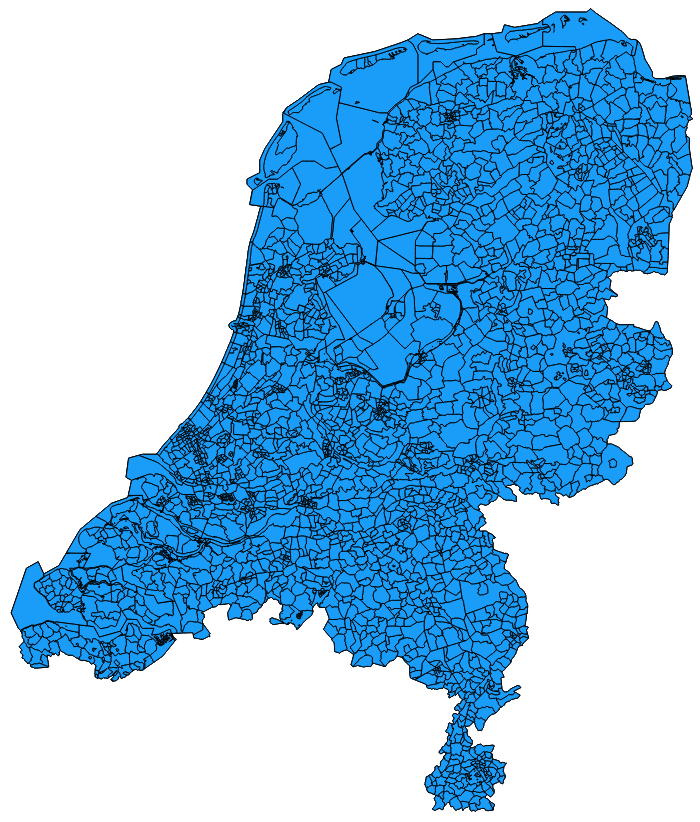
\includegraphics[width=0.5\linewidth]{figs/Neighbourhoods.png}
	\caption{Dataset of neighbourhoods in the Netherlands in 2014 (from \ac{cbs})}
	\label{fig:neighbourhoods}
\end{figure}

\begin{figure}
	\centering
	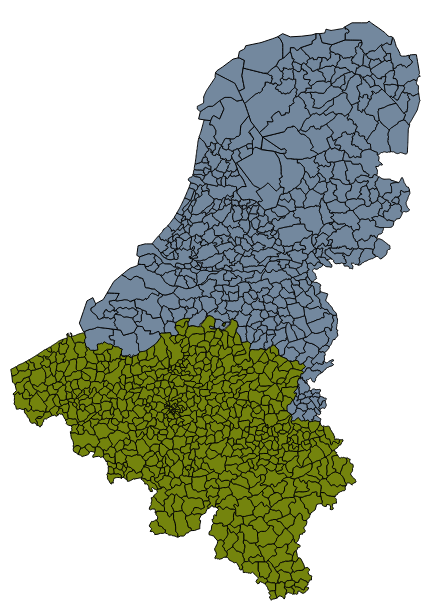
\includegraphics[width=0.5\linewidth]{figs/Municipalities.png}
	\caption{Dataset of municipalities in the Netherlands and Belgium in 2015 (from Dutch cadaster and GADM.org)}
	\label{fig:municipalities}
\end{figure}

\begin{figure}
	\centering
	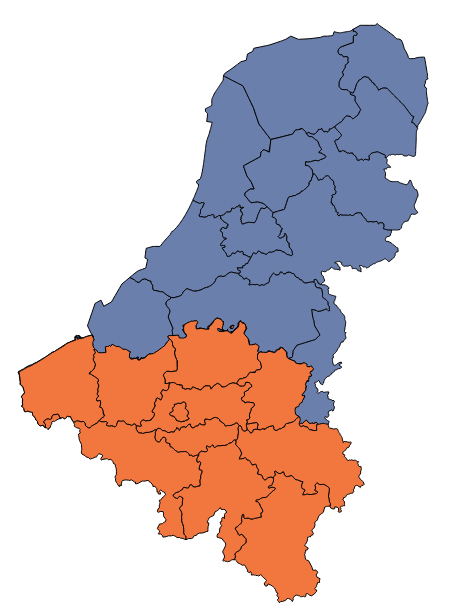
\includegraphics[width=0.5\linewidth]{figs/Provinces.png}
	\caption{Dataset of provinces in the Netherlands and Belgium in 2015 (from Dutch cadaster and GADM.org)}
	\label{fig:provinces}
\end{figure}

\begin{figure}
	\centering
	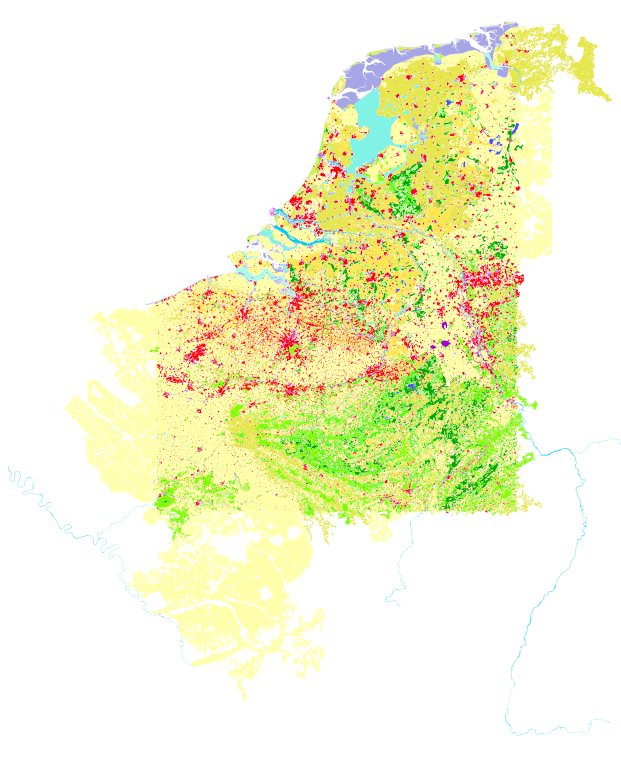
\includegraphics[width=1\linewidth]{figs/CORINE_NL_BE_color.PNG}
	\caption{Dataset of landcover in the Netherlands and Belgium in 2012 (from Copernicus  The European Earth Observation Programme)}
	\label{fig:CORINE}
\end{figure}

\begin{figure}
	\centering
	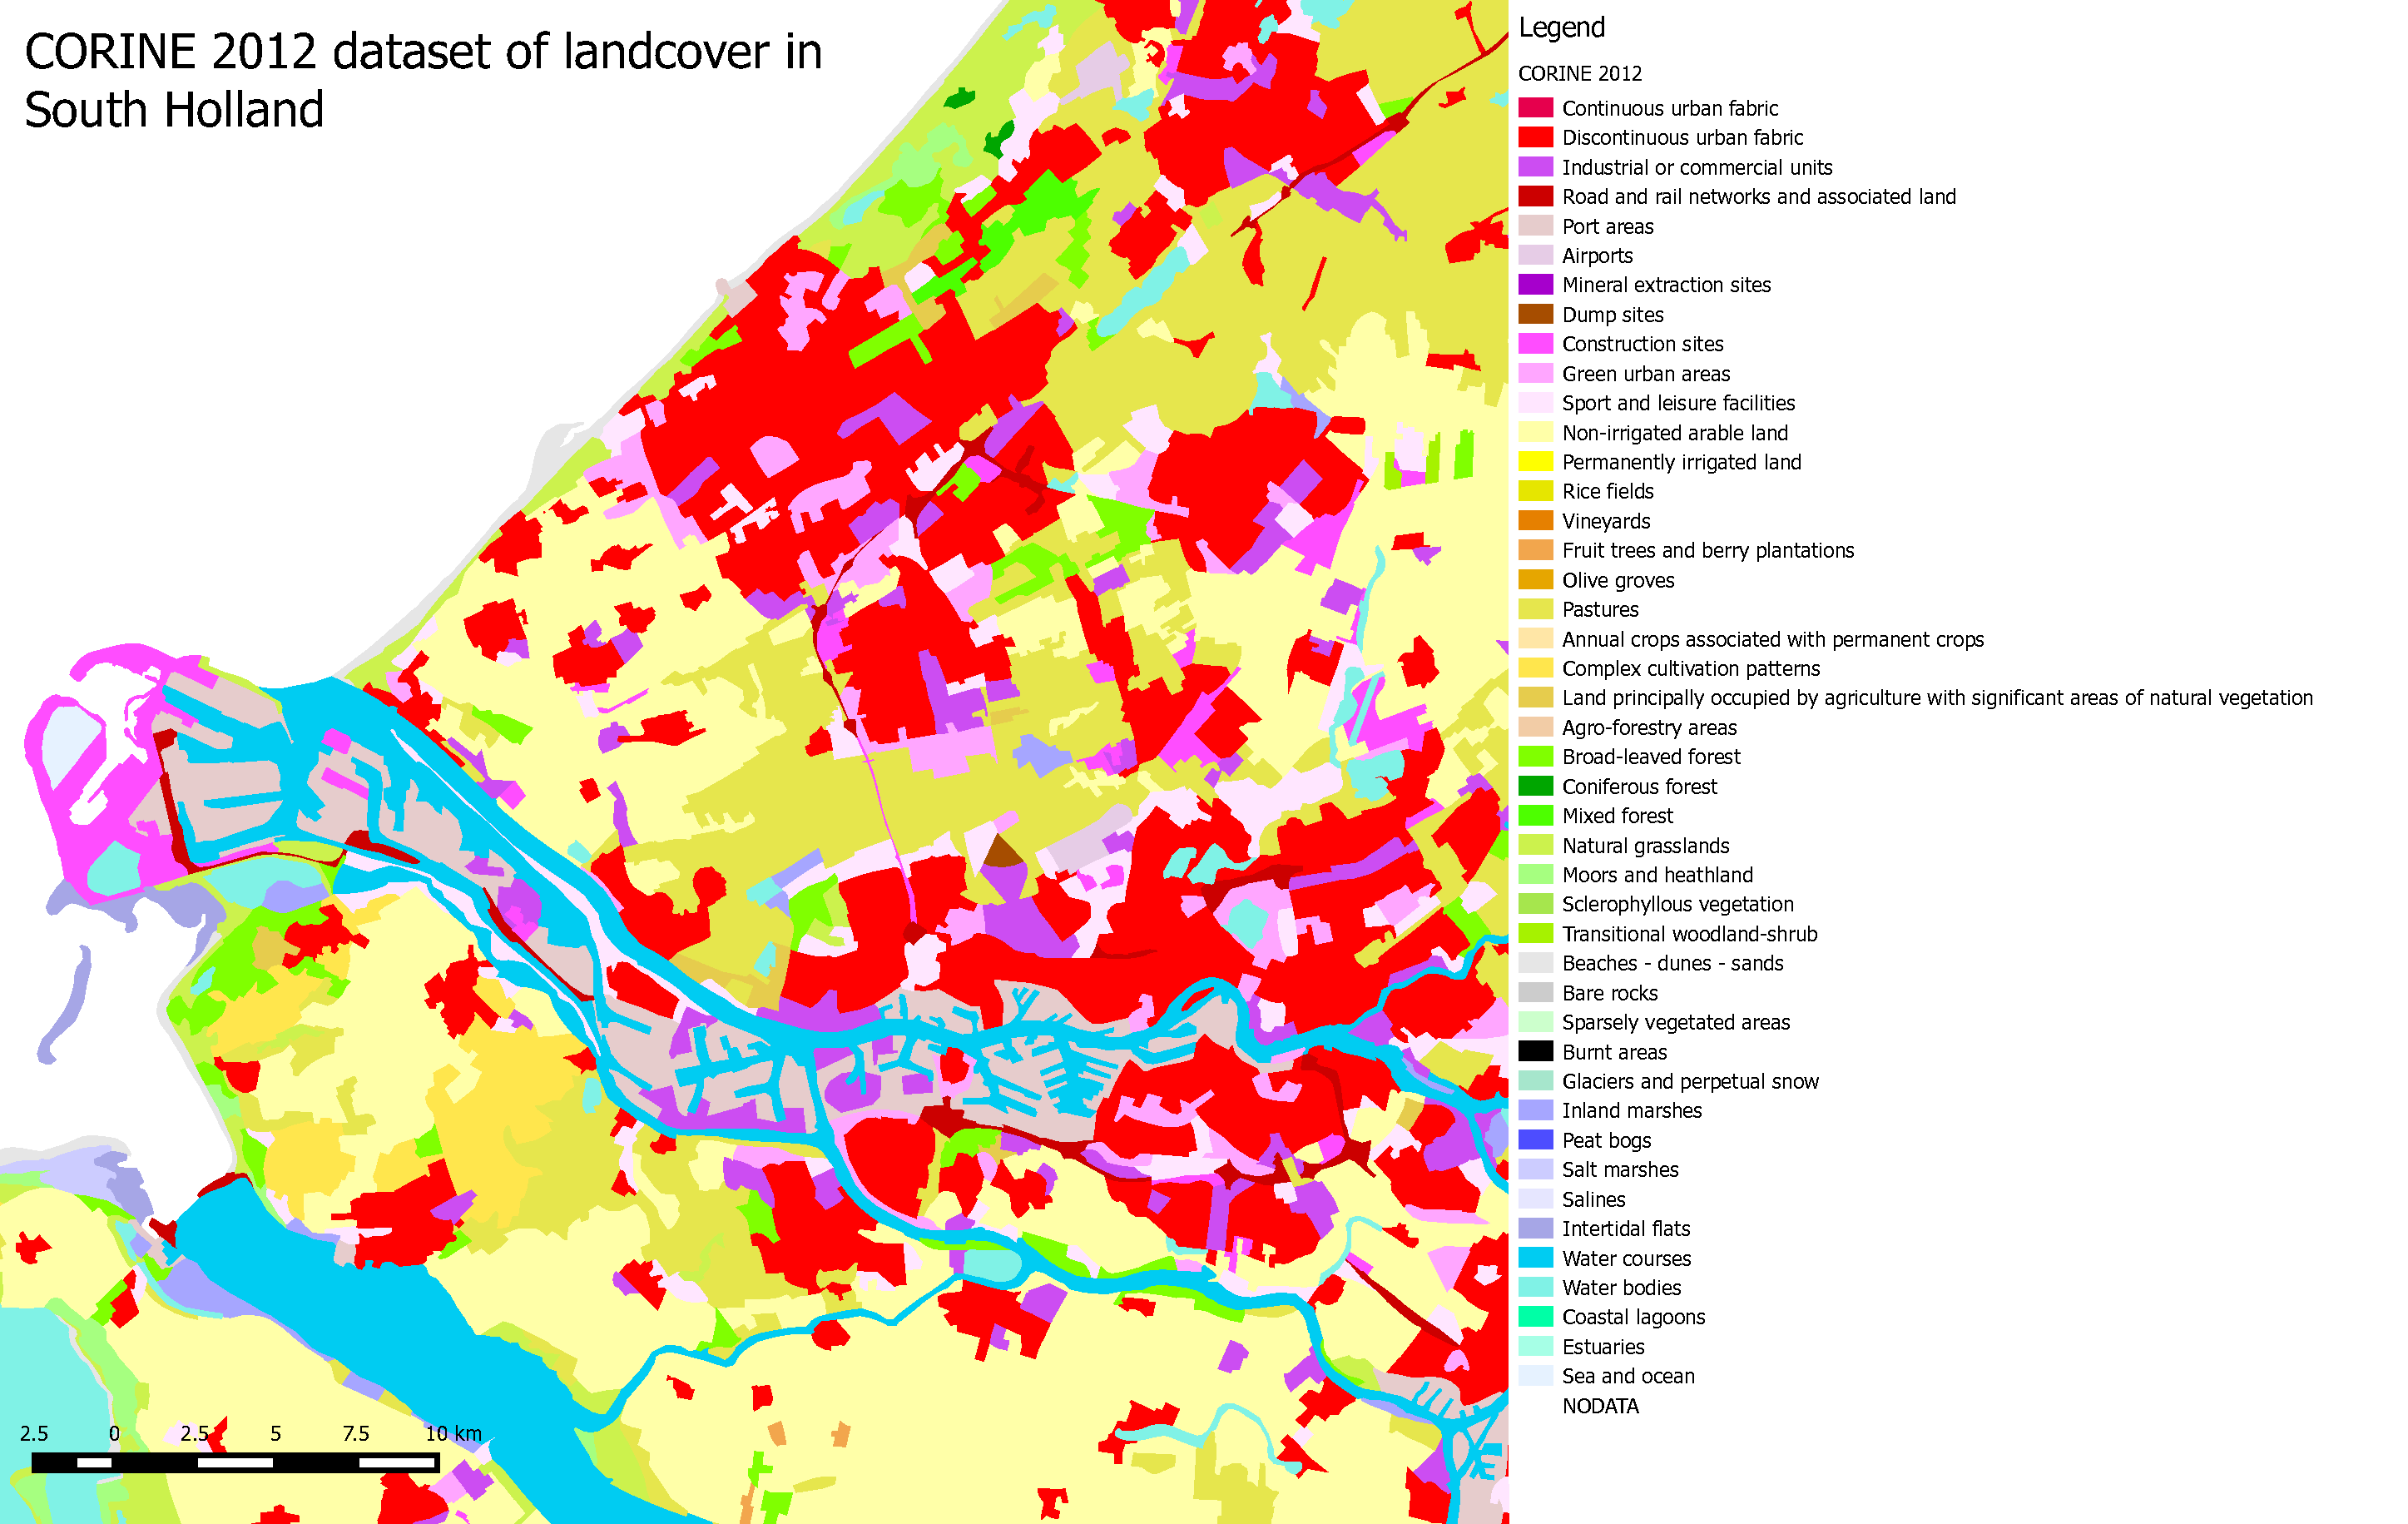
\includegraphics[width=1\linewidth]{figs/CORINE_NL_BE_color_zoom.PDF}
	\caption{Landcover of the province of South Holland (subsection of the dataset from Figure \ref{fig:CORINE})}
	\label{fig:CORINEZOOM}
\end{figure}

Air quality sensor data will be used from the \ac{rivm} (\url{http://inspire.rivm.nl/sos/}) and from the \ac{ircel} (\url{http://sos.irceline.be/}). Both of these organisations have a \ac{sos} where data can be retrieved according to the \ac{swe} standards. The one of the \ac{rivm} has been online since the 21\textsuperscript{st} of August, 2015. \ac{ircel} already made the \ac{sos} available on the first of January, 2011. Figure \ref{fig:RIVMSensor} and Figure \ref{fig:IRCELINESensor} show the sensor networks of both organisations. They provide different kinds of sensor data, such as particulate matter ($PM_{10}$), nitrogen dioxide ($NO^{2}$) and ozone ($O^{3}$). Figure \ref{fig:Sensor} shows one of the sensor locations in the city center of Amsterdam. 


\begin{figure}
	\centering
	\includegraphics[width=0.6\linewidth]{figs/RIVMSensors.png}
	\caption{Webmap by the \ac{rivm} showing their air quality sensor network (\url{http://www.lml.rivm.nl/meetnet})}
	\label{fig:RIVMSensor}
\end{figure}

\begin{figure}
	\centering
	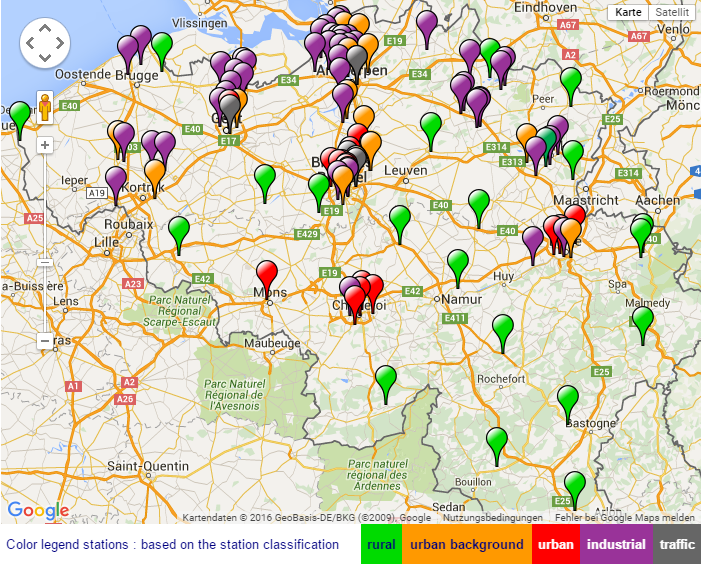
\includegraphics[width=0.6\linewidth]{figs/IRCELINESensors.png}
	\caption{Webmap by \ac{ircel} showing their air quality sensor network (\url{http://www.irceline.be/en/air-quality/measurements/monitoring-stations/})}
	\label{fig:IRCELINESensor}
\end{figure}

\begin{figure}
	\centering
	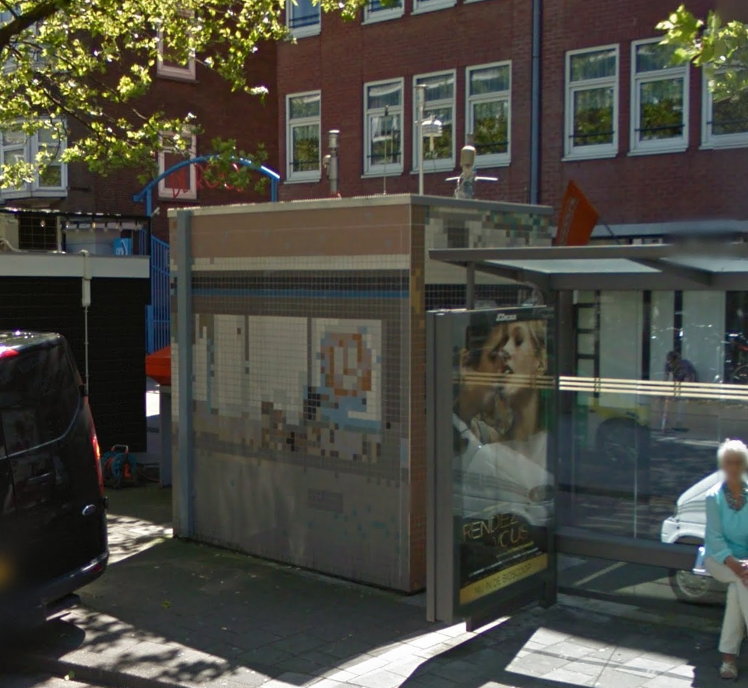
\includegraphics[width=1\linewidth]{figs/SensorAdam.png}
	\caption{Google Streetview image of \ac{rivm} sensor location in Amsterdam}
	\label{fig:Sensor}
\end{figure}


\vbox{%
\subsection{Prototype}
The methods researched in this thesis will be implemented in a prototype. The prototype will be written in the Python programming language and will use a number of Python packages and libraries:\\

\begin{itemize} 
	\item Psycopg2 will be used to connect a Python script to a Postgres database.
	\item Python's \href{http://docs.python-requests.org/en/latest/user/quickstart/}{Request} library will be used for making \ac{http} POST and GET requests. 
	\item For working with \ac{xml} Python's xml package will be used.
	\item To create \ac{rdf} documents the Python library \href{https://rdflib.readthedocs.org/en/stable/}{RDFLib} will be used. 
	\item The scripts will be part of a \ac{wps} using \href{http://pywps.wald.intevation.org/}{PyWPS} 
\end{itemize}}

\subsection{Server}
The prototype will be created on a localhost at first. Once finished it could be hosted on the university server. For the localhost the Apache software will be used, since the PyWPS software requires this. Fuseki Jena is the SPARQL endpoint that is being used (\url{https://jena.apache.org/documentation/serving_data/}).








  

